\documentclass{book}

\usepackage[utf8]{inputenc}
\usepackage[T1]{fontenc}
\usepackage[francais]{babel}
\usepackage{graphicx} 
\usepackage{adjustbox}
\usepackage{fancyref}
\usepackage{hyperref}
\usepackage{url}


\title{%
  Projet de Sciences des Données \\
  \large Explotation d'images satellites haute-résolution \\pour la prevision d'indicateurs socio-économiques \\
    }

\author{\textsc{Youcef} - \textsc{Kacer}}
\date{9 Septembre 2016}

\begin{document}
 
\maketitle

\tableofcontents

\frontmatter
\chapter{Introduction}
Ce document présente le pré-traitement des images du satellite Landsat-8 en vue de la prédiction d'indicateurs socio-économiques (à 
priori la densité de population dans un premier temps). Il s'agit de montrer comment, pour un territoire donné,
importer les images depuis le site de l'$USGS$ (\begin{itshape}U.S. Geological Survey\end{itshape}) \cite{landsat8}, en supprimer les doublons, et ne conserver 
que celles de meilleure qualité.
Ensuite, nous verrons comment exploiter les méta-données liées à chaque image afin de les projeter sur un plan, cela de manière conforme
à la norme $UTM$ (\begin{itshape}Universe Transverse Mercator\end{itshape}).
Puis, nous verrons comment former des combinaisons de bandes d'images pertinentes et en doubler la résolution (de 30m à 15m) via
la technique de \og pan-sharpening \fg{}.
\mainmatter

\chapter{Importation des images Landsat-8}
\section{Téléchargement}

L'interface du site de l'USGS permet de rechercher des images contenues dans une zone à délimiter via des points repérés par 
leur latitude et longitude \ref{selection}.\\

\begin{figure}[H]
\begin{center}
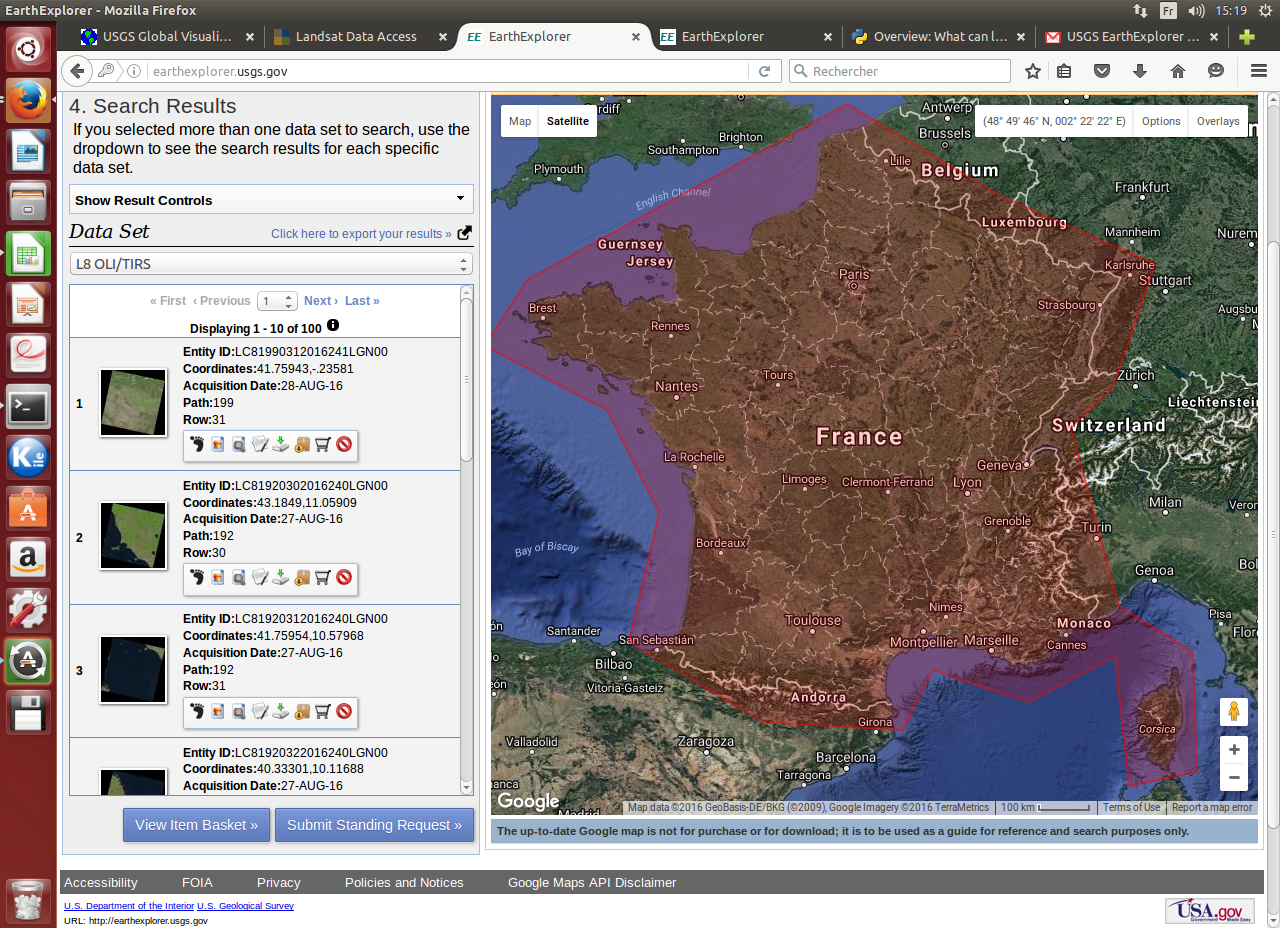
\includegraphics[scale=0.3]{images/polygon_selection.png}
\end{center}
\caption{Selection d'un polygone (en rouge) sur l'interface du site de l'$USGS$}
\label{selection}
\end{figure}

\clearpage

Plusieurs critères sont disponibles et que nous allons exploiter :\\

\begin{itemize}

\item[-] Contr\^{o}ler la couverture nuageuse (inférieure à 10\%).
\item[-] Contr\^{o}ler la période d'acquistion (privilégier les acquisitions de jour).
\item[-] Renseigner des bornes d'acquisition en temps (prendre une large étendue temporelle pour être s\^{o}r de couvrir tout le territoire)

\end{itemize}

Ainsi, le résultat de notre recherche peut être exporté dans un fichier au format .csv, contenant pour chaque image, plus d'une 
cinquantaine d'attributs, dont nous affichons ceux qui nous seront utiles \ref{attributs}.\\

\begin{table}
\begin{center}
\begin{adjustbox}{max width=\textwidth}
\begin{tabular}{|c|c|c|c|c|c|c|c|c|c|c|c|c|c|c|c|}
\hline
Landsat Scene Identifier&WRS Path&WRS Row&Day/Night&Scene Cloud Cover&Center Latitude dec&Center Longitude dec&NW Corner Lat dec&NW Corner Long dec&NE Corner Lat dec&NE Corner Long dec&SE Corner Lat dec&SE Corner Long dec&SW Corner Lat dec&SW Corner Long dec&Download Link\\
\hline
LC81950282013364LGN00& 195& 028&DAY&7.44&46.02984&7.38892&47.09274&6.48836&46.65946&8.91959&44.95062&8.24933&45.3793&5.89077&http://earthexplorer.usgs.gov/download/options/4923/LC81950282013364LGN00\\
\hline
LC81950292013364LGN00& 195& 029&DAY&3.2&44.60804&6.87298&45.66897&5.9903&45.24275&8.36095&43.53106&7.71815&43.95338&5.41529&http://earthexplorer.usgs.gov/download/options/4923/LC81950292013364LGN00\\
\hline
LC81950302013364LGN00& 195& 030&DAY&.8&43.18461&6.37702&44.24369&5.51195&43.82416&7.82483&42.10976&7.20688&42.52603&4.95724&http://earthexplorer.usgs.gov/download/options/4923/LC81950302013364LGN00\\
\hline
LC81940312013357LGN00& 194& 031&DAY&10.05&41.75982&7.44724&42.81727&6.59873&42.40382&8.85813&40.68687&8.26289&41.09763&6.06252&http://earthexplorer.usgs.gov/download/options/4923/LC81940312013357LGN00\\
\hline
LC81930302013350LGN00& 193& 030&DAY&.53&43.18488&9.47096&44.24392&8.60693&43.82465&10.91796&42.11008&10.29987&42.52607&8.05201&http://earthexplorer.usgs.gov/download/options/4923/LC81930302013350LGN00\\
\hline
LC81930312013350LGN00& 193& 031&DAY&3.83&41.75944&8.99273&42.81693&8.14431&42.40341&10.40366&40.68644&9.80829&41.09728&7.60796&http://earthexplorer.usgs.gov/download/options/4923/LC81930312013350LGN00\\
\hline
LC81950302013348LGN00& 195& 030&DAY&6.14&43.18481&6.37736&44.24394&5.51273&43.82444&7.82497&42.10994&7.20687&42.52616&4.95783&http://earthexplorer.usgs.gov/download/options/4923/LC81950302013348LGN00\\
\hline
LC81990262013344LGN00& 199& 026&DAY&1.33&48.86642&2.30469&49.93403&1.36584&49.4846&3.93152&47.78194&3.19748&48.22517&.71549&http://earthexplorer.usgs.gov/download/options/4923/LC81990262013344LGN00\\
\hline
LC81990302013344LGN00& 199& 030&DAY&2.96&43.18467&.19295&44.24396&-.67281&43.82406&1.64167&42.10966&1.0236&42.52629&-1.22763&http://earthexplorer.usgs.gov/download/options/4923/LC81990302013344LGN00\\
\hline
..&..&..&..&..&..&..&..&..&..&..&..&..&..&..&..\\
\hline
\end{tabular}
\end{adjustbox}
\end{center}
\caption{Images Landsat-8 et méta-données}
\label{attributs}
\end{table}

On énumère ci-après les attributs pertinents du fichier .csv obtenu et leur utilité :\\

\begin{itemize}

\item[-] Nom formatté de l'image LXSPPPRRRYYYYDDDGSIVV (L = Landsat, X = type du senseur, S = Satellite (ici landsat8),
PPP = WRS path, RRR = WRS row, YYYY = Année, DDD = jour de l'année, GSI = identifiant de station au sol, 
VV = numéro de version d'archivage)
\item[-] \begin{itshape}WRS path\end{itshape} et \begin{itshape}WRS row\end{itshape} sont des coordonnées qui définissent un pavage de la surface terrestre par le satellte (voir \ref{wrs}
pour un pavage $WRS$ de l'état de $Virginie$, $USA$). Ce sont ces deux attributs qui permettent de retirer les doublons. Pour
plusieurs images ayant les mêmes coordonnées $WRS$, on conserve celle de couverture nuageuse minimum.
\item[-] Jour/nuit
\item[-] Couverture nuageuse en \%
\item[-] Les latitudes et longitudes correspondant au centre et aux quatres coins de l'image
\item[-] Le lien vers le téléchargement du dataset de l'image

\end{itemize}

\begin{figure}[H]
\begin{center}
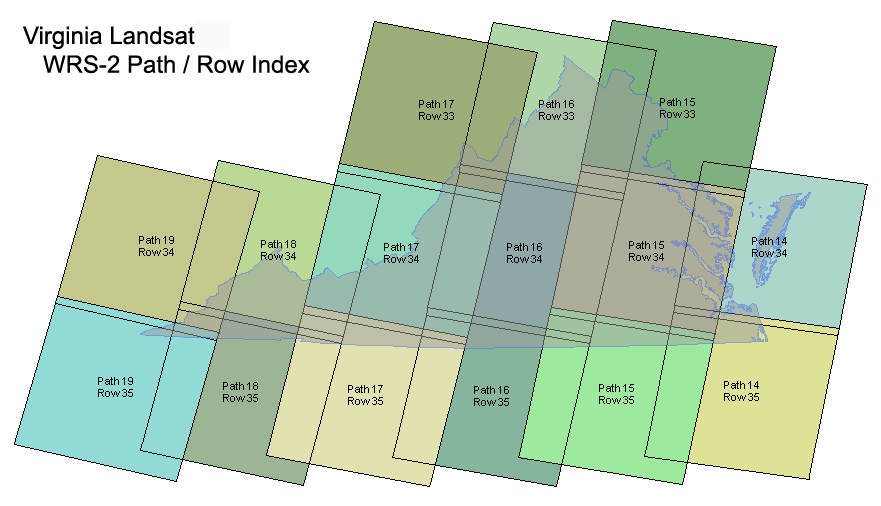
\includegraphics[scale=0.4]{images/wrs.png}
\end{center}
\caption{pavage $WRS$ de l'état de $Virginie$, $USA$ \cite{Virginia}}
\label{wrs}
\end{figure}

\clearpage

\section{Projection}

Nous avons donc une liste d'identifiants d'images avec leurs coordonnées en latitude et longitude, que nous pouvons télécharger.\\
Nous avons vu que ces données peuvent être obtenues sans redondance, prises de jour, avec une couverture nuageuse minimale.\\
Cependant, il reste à verifier que ces données couvrent bien le territoire voulue, pour cela nous allons projeter les images obtenues
sur un plan en utlisant la convention $UTM$ \cite{wiki:utm}.\\
Cette convention divise la surface terreste en zones délimitées par les méridiens (espacées de 6 degrés) et 
les latitudes (espacées de 8 degrés) \ref{utm}.
\begin{figure}[H]
\begin{center}
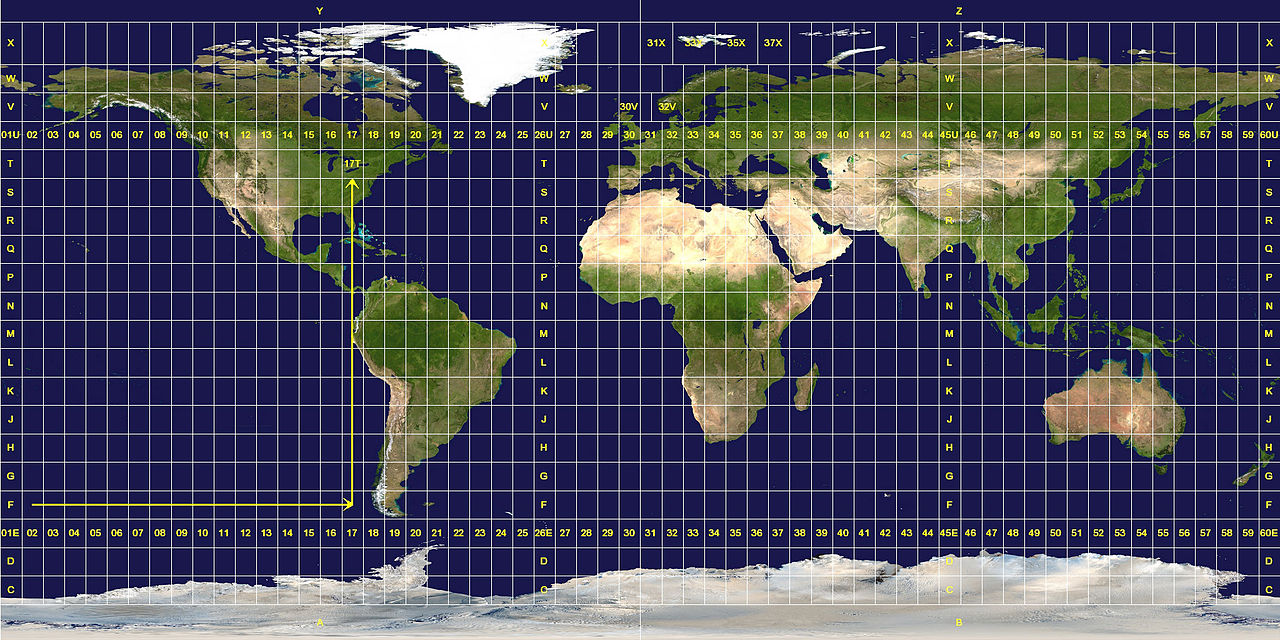
\includegraphics[scale=0.3]{images/utm_zones.jpg}
\end{center}
\caption{Division de la surface terrestre en zones ($UTM$) \cite{wiki:utm}}
\label{utm}
\end{figure}

\clearpage

Pour une zone donnée, les couples ($latitude$,$longitude$) sont projetés en tenant compte de l'aspect ellipsoidal local de la terre 
(la convention $WGS84$ définie les dimensions de l'ellipse).\\
Les coordonnées ($x$,$y$) obtenues sont en mètres par rapport à une origine virtuelle différente pour chaque zone. De ce fait, la distance
entre un point d'une zone et un point d'une autre zone n'a aucun sens et chaque zone a son propre système de projection.\\
Cette distance a cependant un sens si toutes les cordonnées ($longitude$,$latitude$) sont converties en coordonnées ($x$,$y$) suivant
le système de projection d'une même zone donnée, aux effets de distorsion prêt.\\
C'est cette simplification que nous allons adopter : pour chaque territoire, on utilisera le système de projection de la zone centrale.
Par exemple, pour notre exemple du territoire français, nous allons projeté les ($longitude$,$latitude$) en prenant le système de projection
de la zone $31T$ \ref{utm_france} :

\begin{figure}[H]
\begin{center}
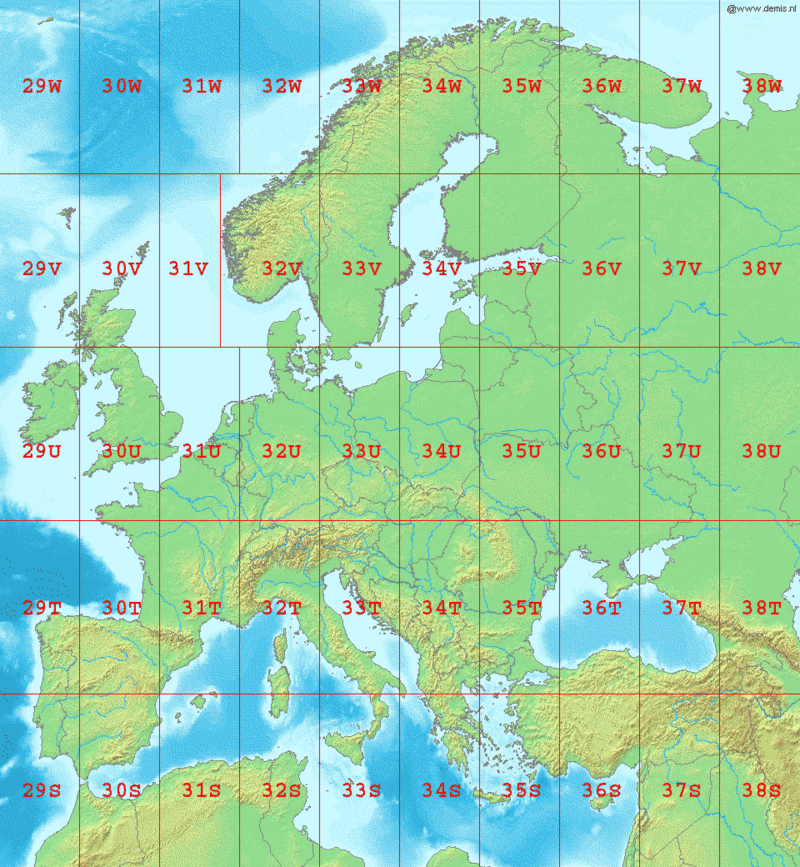
\includegraphics[scale=0.3]{images/utm_zones_europe.png}
\end{center}
\caption{Division de continent européen en zones ($UTM$) \cite{wiki:utm}}
\label{utm_france}
\end{figure}

\clearpage

Ainsi, nous avons projeté les résultats de notre recherche concernant le territoire français \ref{projection_france}, en utilisant 
la package $utm$ sur $python$ \cite{utm_package}.

\begin{figure}[H]
\begin{center}
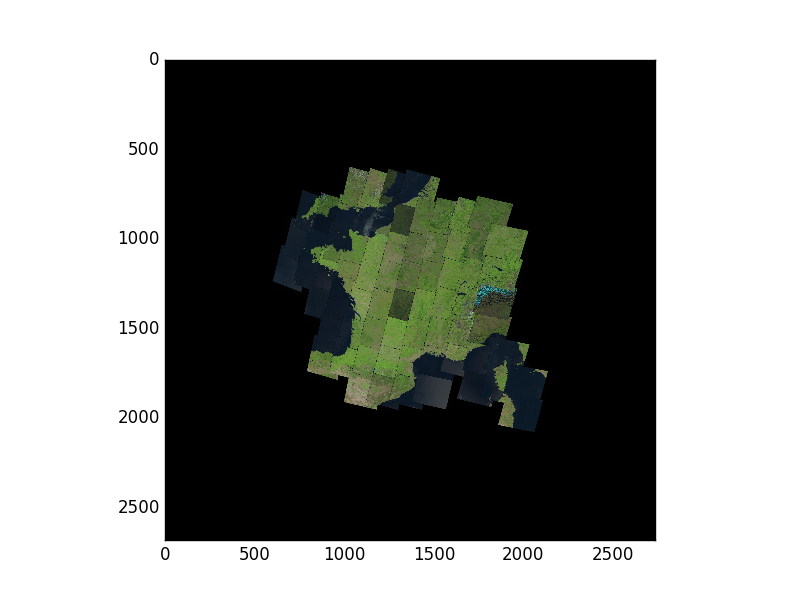
\includegraphics[scale=0.8]{images/projection_france.png}
\end{center}
\caption{Projection $UTM$ d'images Landsat-8 du territoire $France$}
\label{projection_france}
\end{figure}

On remarque que tout le territoire français est couvert avec une couverture nuageuse quasi-absente.

\clearpage

Nous avons réitére le processus de selection des images sur le site de l'$USGS$ et effectuer leur projection,
pour d'autres territoires à divers endroits du globe \ref{projection_uruguay},\ref{projection_kenya},\ref{projection_newzealand},\ref{projection_usa}:
\begin{figure}[H]
\begin{center}
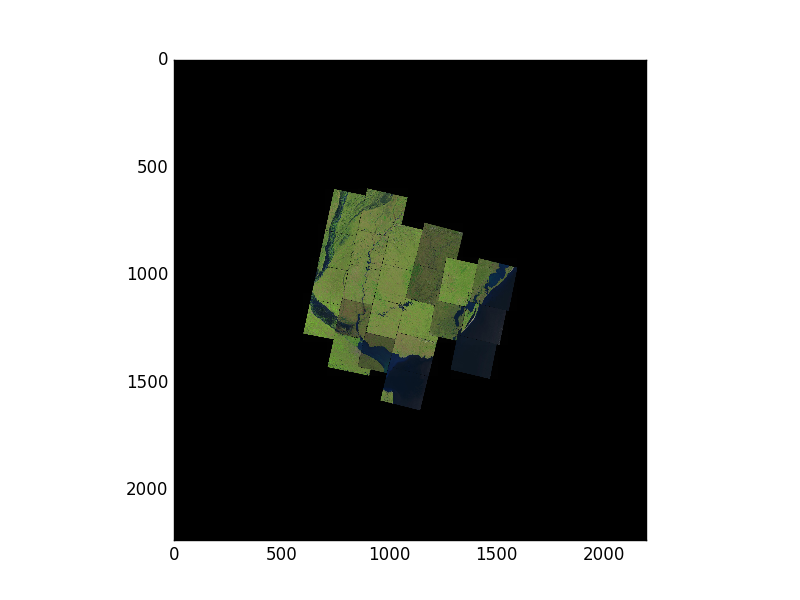
\includegraphics[scale=0.8]{images/projection_uruguay.png}
\end{center}
\caption{Projection $UTM$ d'images Landsat-8 du territoire $Uruguay$}
\label{projection_uruguay}
\end{figure}
\begin{figure}[H]
\begin{center}
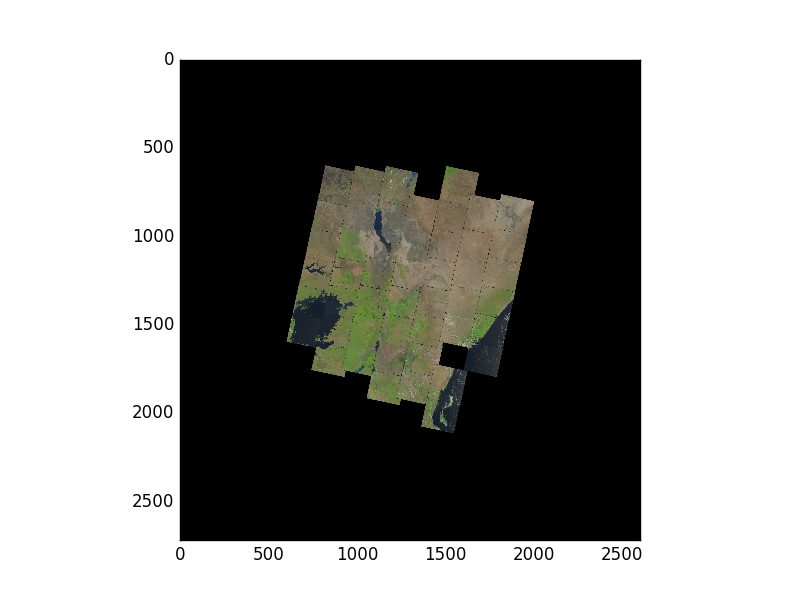
\includegraphics[scale=0.8]{images/projection_kenya.png}
\end{center}
\caption{Projection $UTM$ d'images Landsat-8 du territoire $Kenya$}
\label{projection_kenya}
\end{figure}
\begin{figure}[H]
\begin{center}
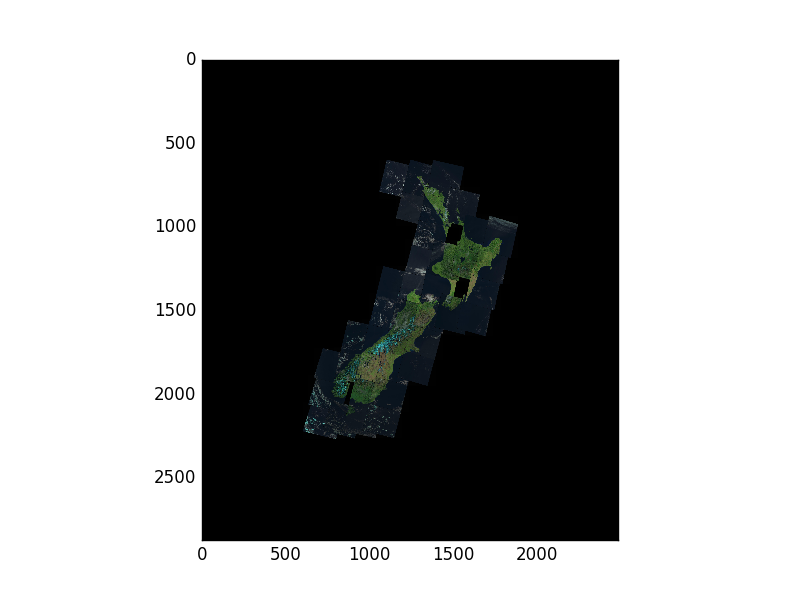
\includegraphics[scale=0.8]{images/projection_newzealand.png}
\end{center}
\caption{Projection $UTM$ d'images Landsat-8 du territoire $Nouvelle$-$Zelande$}
\label{projection_newzealand}
\end{figure}
\begin{figure}[H]
\begin{center}
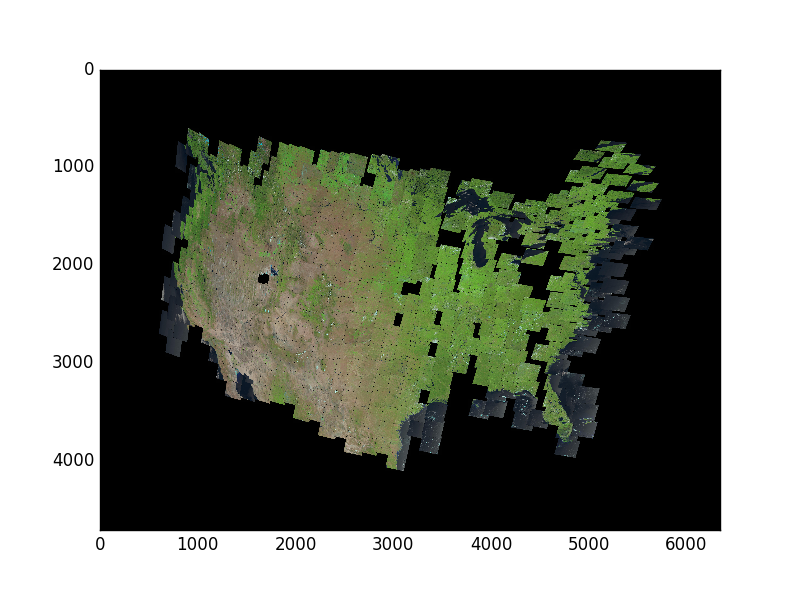
\includegraphics[scale=0.8]{images/projection_usa.png}
\end{center}
\caption{Projection $UTM$ d'images Landsat-8 du territoire $USA$}
\label{projection_usa}
\end{figure}

\clearpage

On remarquera que pour certains terrioires comme celui ds $USA$ ou celui de \begin{itshape}Nouvelle-Zelande\end{itshape}, 
le territoire n'est pas totalement couvert. En effet, les requ\^{e}tes sur le site de l'$USGS$ renvoit un maximum 
de 100 images, et il se peut donc que toutes les images ne couvrent pas toute la zone délimitée. 
Mais, on peut palier à cela en augmentant ce maximum 
ou en effectuant plusieurs recherches du même territoire pour différentes année qu'on concatène ensuite.\\

\chapter{Pré-traitement des images}
\section{Combinaison de bandes spectrales}

A ce stade, nous avons donc une liste d'url vers des images Landsat-8 couvrant un certain territoire.\\
Chaque image est en fait un dataset de 11 canaux, 9 dans le visible et 2 dans l'infra-rouge.\\
L'illustration \ref{lc8_bands} montre les bandes spectrales des 11 canaux pour les satellites 
Landsat-7 (en bas) et Landsat-8 (en haut):
\begin{figure}[H]
\begin{center}
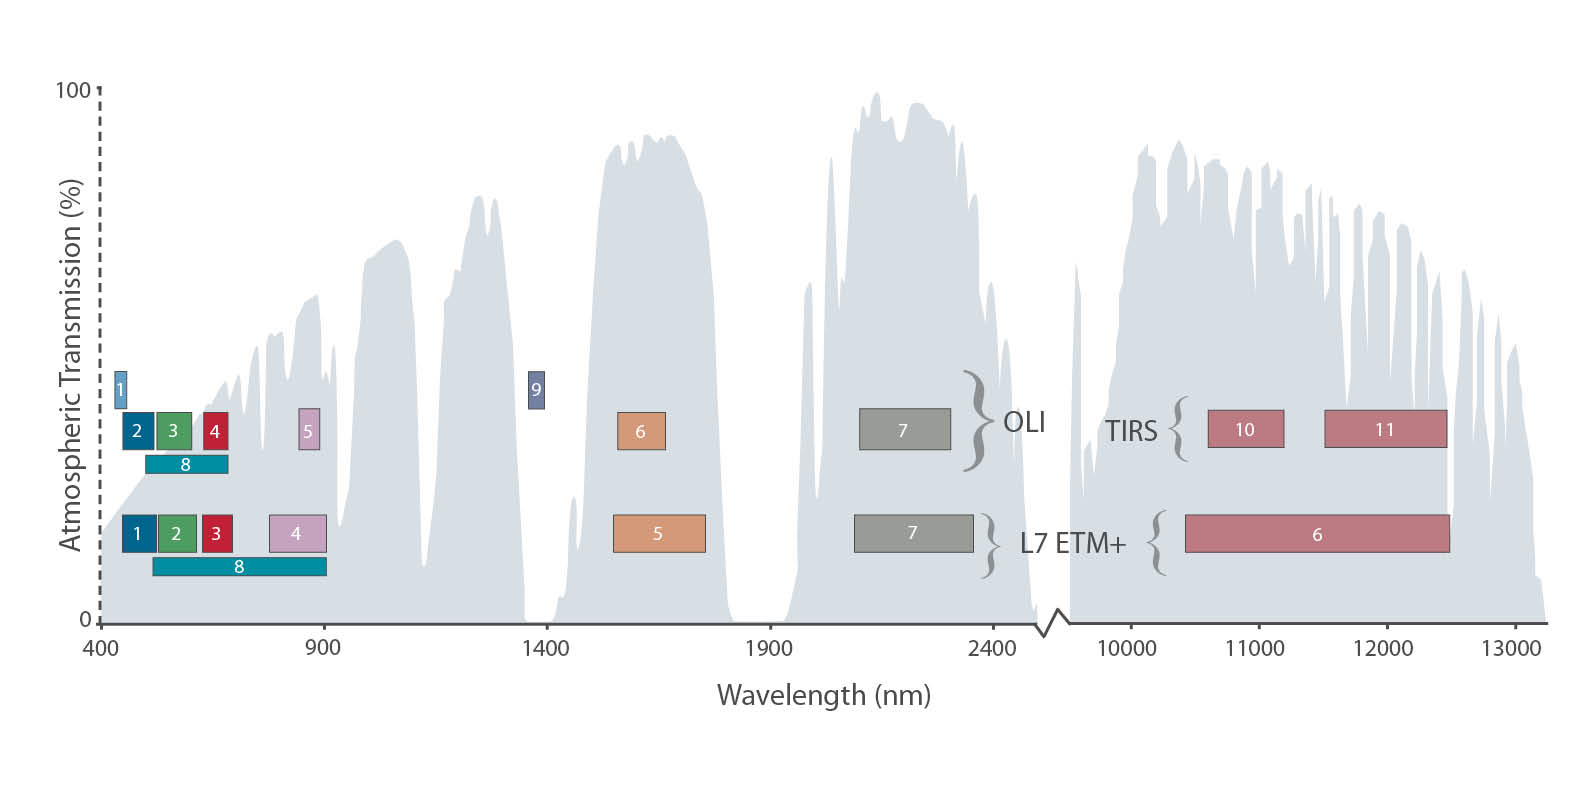
\includegraphics[scale=0.2]{images/landsat8_bands.jpg}
\end{center}
\caption{Bandes spectrales des différents canaux spectraux pour les satellites Landsat-7 et Landsat-8 \cite{landsat8}}
\label{lc8_bands}
\end{figure}

\clearpage

Certaines combinaisons bien spécifiques de bandes peuvent apporter de l'information, comme le montre le tableau \ref{combinaison}
tiré de \cite{esri}:\\

\begin{table}
\begin{center}
\begin{tabular}{|c|c|c|c|}
\hline
Natural Color & 4 , 3 , 2\\
\hline
False Color (urban) & 7 , 6 , 4\\
\hline
Color Infrared (vegetation) & 5 , 4 , 3\\
\hline
Agriculture & 6 , 5 , 2\\
\hline
Atmospheric Peration & 7 , 6 , 5\\
\hline
Healthy Vegetation & 5 , 6 , 2\\
\hline
Land/Water & 5 , 6 , 4\\
\hline
Natural With Atmospheric Removal & 7 , 5 , 3\\
\hline
Shortwave Infrared & 7 , 5 , 4\\
\hline
Vegetation Analysis & 6 , 5 , 4\\
\hline
\end{tabular}
\end{center}
\caption{Combinaisons possibles à 3 canaux}
\label{combinaison}
\end{table}
\clearpage

Ces bandes couvrent approximativement un périmètre de 185km dans la direction Nord-Sud et 185km
dans la direction Est-Ouest, pour une résolution de 30 mètres (soit des images d'environ 8000 sur 8000 pixels).\\
La figure \ref{color} presente la combinaison de ces trois bandes Rouge, Vert, Blue, et donc l'image couleur resultante 
(ainsi qu'un zoom autour de l'\begin{itshape}Ile-de-France\end{itshape}).\\
La figure \ref{vegetation} presente la combinaison des trois bandes 6,5,4 qui permet l'analyse de la végétation.\\


\begin{figure}[H]
\begin{center}
\includegraphics[scale=0.03]{images/paris_rgb.png}
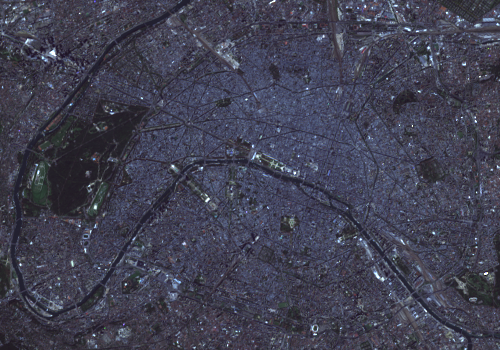
\includegraphics[scale=0.5]{images/paris_rgb_zoom.png}
\end{center}
\caption{image couleur Lansat-8 (bandes 4,3,2), région autour de $Paris$ $(France)$ + zoom}
\label{color}
\end{figure}


\begin{figure}[H]
\begin{center}
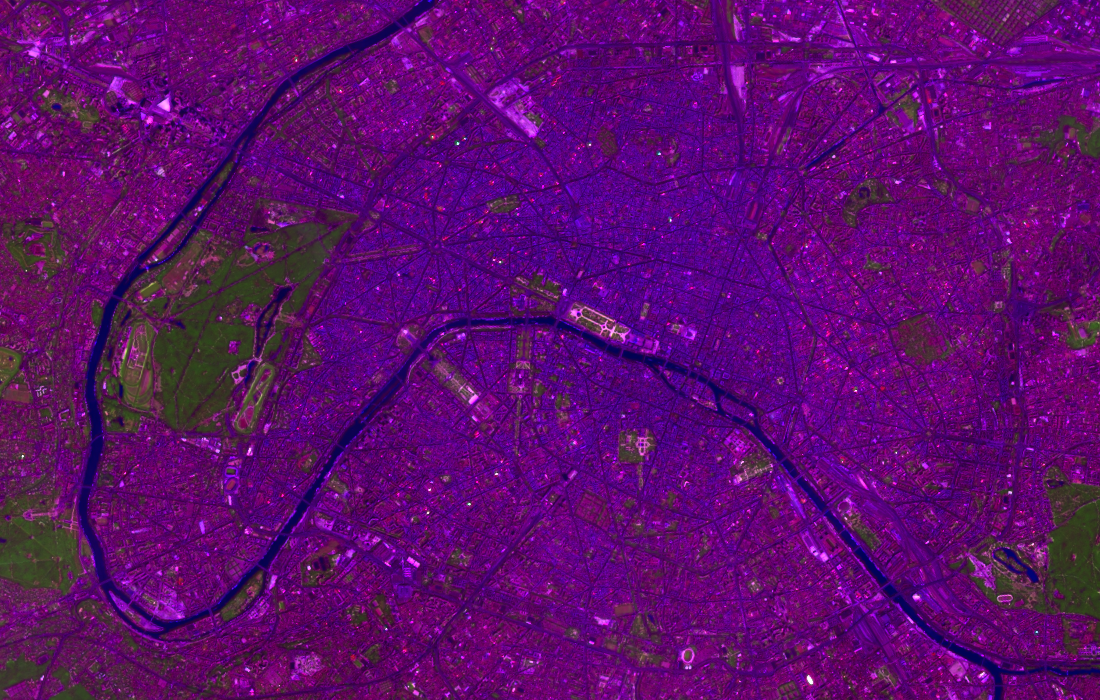
\includegraphics[scale=0.3]{images/paris_vegetal_zoom_pansharpened.png}
\end{center}
\caption{image végétale Lansat-8 (bandes 6,5,4), région autour de $Paris$ $(France)$}
\label{vegetation}
\end{figure}

\clearpage

\section{Pan-sharpening}

Parmi les 11 bandes, la bande 8 est la seule présentant une résolution de 15m au lieu de 30m. Elle est utilisé pour améliorer la résolution
des combinaisons de bandes.\\
Ainsi la figure \ref{pan-sharpen} montre la différence entre l'image couleur à 30m de résolution et cella à 15m obtenue par pan-sharpening.
Pour calculer cette image, on utilise le package Linux \begin{itshape}landsat-util\end{itshape} \cite{dans-gdal}.

\begin{figure}[H]
\begin{center}
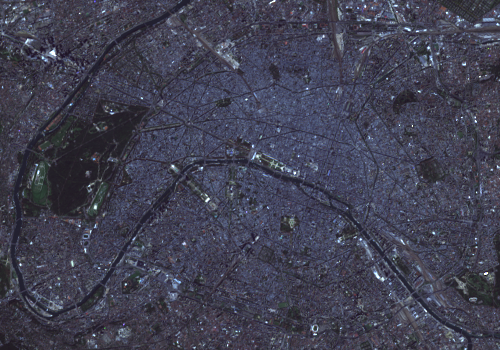
\includegraphics[scale=0.4]{images/paris_rgb_zoom.png}
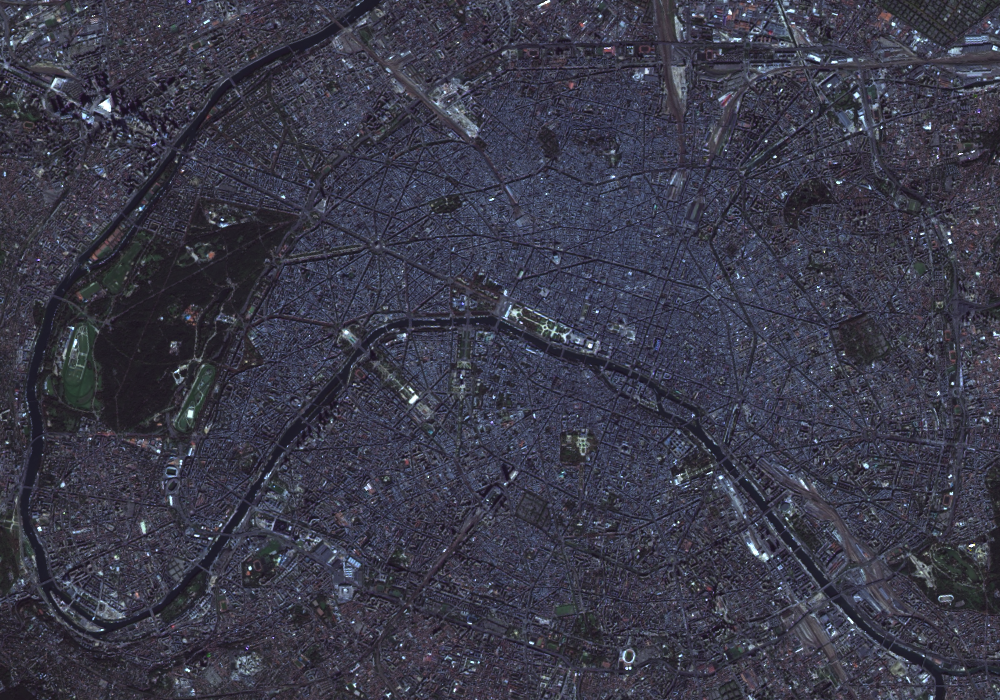
\includegraphics[scale=0.2]{images/paris_rgb_zoom_pansharpened.png}
\end{center}
\caption{image couleur Landsat-8 et son pan-sharpening, $Paris$ $(France)$}
\label{vegetation}
\end{figure}

\clearpage

\backmatter

\listoftables

\listoffigures

\bibliographystyle{alpha}
\bibliography{biblio}

\end{document}